\documentclass[11pt,a4paper]{article}
\usepackage[utf8]{inputenc}
\usepackage[T1]{fontenc}
\usepackage{amsmath,amssymb,amsthm}
\usepackage{graphicx}
\usepackage[margin=2.5cm]{geometry}
\usepackage{hyperref}
\usepackage{xcolor}
\usepackage{booktabs}
\usepackage{authblk}
\usepackage{cite}
\usepackage{enumitem}
\hypersetup{colorlinks=true,linkcolor=blue,citecolor=blue,urlcolor=blue}

\title{\textbf{Discrete Drainage Dynamics II:\\
Cascade-Throttled Drainage and\\
a Schwarzschild-Like Time-Dilation Factor}}
\author[1]{Stanislas Dewavrin}
\affil[1]{Independent researcher \\ \texttt{dewavrin.iphone@gmail.com}}
\date{April 2026}

\begin{document}
\maketitle

\begin{abstract}
\noindent
\textbf{Discrete Drainage Dynamics (DDD) is an analogue-substrate
programme.} It does not contest General Relativity, the
Newtonian limit, or the Standard Model: those are empirical
anchors that any analogue must reproduce in the appropriate
continuum and regime limits. DDD asks the more modest,
exploratory question of whether some of the \emph{forms} that
appear fundamental in current physics can be made mechanically
legible inside a deliberately simpler discrete toy substrate.
The present paper studies the static spherical gravitational
sector of that analogue.

Paper~I introduced DDD as a reserve-flux framework with a
mobility function $\mu(R)$ that the framework left open, and
studied the constant-mobility baseline $\mu \equiv 1$ that
recovers the form of Newton's $1/r$ at leading order in the continuum limit of the analogue substrate. Here we close that gap.
Within the class of local emission-capacity rules, we show that
four operational axioms --- locality, internal conservation,
empty-reserve extinction, and additivity of independent reserve
packets (L4) --- uniquely select the source-side mobility
$\mu(R) = R/R_0$ via the Cauchy functional equation and standard
regularity. \emph{The construction rests on two substantive
hypotheses not derived from deeper principles: (H1) the
additivity axiom (L4), and (H2) the bandwidth identification
$d\tau/dt = R/R_0$ of effective proper time with the
reserve-normalised bandwidth (introduced in Sec.~\ref{sec:setup}).
Under these two hypotheses and the locality axioms (L1)--(L3),
the source-side mobility is forced and the Schwarzschild form
follows; the microscopic origin of (H1) and (H2) is the
principal open problem of the construction and is left to
future work.} The directional flux on a link is therefore modulated
by the bandwidth available at the source node, with no
receiver-side throttle in the emission-capacity sector. Under
this axiomatically selected mobility, the steady-state field
around a point sink satisfies the algebraic identity $\nabla^2(R^2) = 0$ in
the continuum limit, away from the sink. The unique
spherically-symmetric solution with $R \to R_0$ at infinity
is $R/R_0 = \sqrt{1 - \beta/r}$, with $\beta$ fixed by the
source strength. This is the form of the Schwarzschild static
clock-rate factor, $\sqrt{1 - 2GM/c^2 r}$, under the
identification $\beta = 2GM/c^2$. Combined with the
operational identification of effective proper time with local
bandwidth ($d\tau/dt = R/R_0$), the model reproduces a
Schwarzschild-like static clock-rate factor in the continuum
spherical solution, conditional on the additive
emission-capacity axioms and the bandwidth identification. We verify the result numerically.
From the same structural input we extract the functional form
of Newton's gravitational constant $G$ in terms of the local
rule parameters $(\kappa, \alpha, R_0)$ and the lattice scale,
together with a single Planck-anchored dimensionless constraint
$\kappa/(\alpha R_0) = 4\pi$. \emph{This Planck-anchoring
condition is a consistency requirement under the Planck
identification, not an independent prediction of $G$.} We do not
predict the SI value of
$G$ (the absolute lattice scale must be anchored externally),
nor do we derive the speed of light $c$, the spatial part of
the metric, or the Einstein field equations.
\end{abstract}


\noindent\fbox{\parbox{0.96\textwidth}{\small
\textbf{What this paper makes mechanically legible.}
GR predicts the Schwarzschild form $g_{tt} \propto -(1-\beta/r)$
with metric precision but supplies no mechanism for \emph{why}
clocks tick slow near a mass, and produces a curvature
singularity at $r = 0$ where the continuum theory breaks down.
\emph{This paper} reads $g_{tt}$ as a substrate-level bandwidth
ratio $R/R_0$ under source-side throttling: nodes near a sink
literally have less bandwidth available, slowing their internal
event rate. The would-be singularity is replaced by a
\emph{bandwidth horizon} where Paper~I's discrete rate-limiter
activates. \textbf{Leverage:} the form of $g_{tt}$ acquires a
mechanism, and GR's curvature singularity is regularised by
the discrete substrate --- the marker that the analogue can
do better than the continuum where the latter signals its own
breakdown.
}}
\bigskip


\section{Main claims and scope}
\label{sec:claims}

\paragraph{Programme positioning and analogue framing.}
Before stating the claims of this paper we recall the position
of the entire DDD programme. DDD is an analogue-substrate
programme: General Relativity, the Newtonian limit, and the
Standard Model are not contested; they are the empirical
anchors any analogue must reproduce in the appropriate
continuum and regime limits. The aim of this paper is not to
replace GR but to ask whether the \emph{form} of the
Schwarzschild static clock-rate factor can be made mechanically
legible inside a deliberately simpler discrete substrate with
finite reserves and local update rules. The results are
internal to the analogue and conditional on the stated
hypotheses (H1) and (H2); they do not claim to derive the
underlying physical law. Any deviation between the analogue
and the empirical theories is a falsifier of the analogue, not
of the empirical theories.


\begin{enumerate}
\item \textbf{Bandwidth identification.} Within the rule of
Paper~I, the maximum directional flux a node $i$ can push out
is $\alpha R_i$, set by the locally available reserve. We
identify the dimensionless ratio $R_i/R_0$ with the local rate
of effective proper time:
\[
\frac{d\tau_i}{dt} \;=\; \frac{R_i}{R_0}.
\]
This identification is operational, not derived; it states
that a node's local rate of activity per coordinate tick is
proportional to its available reserve.

\item \textbf{Source-side bandwidth mobility, derived from
four locality axioms.} Within the rule of Paper~I, the local
emission capacity $C(R)$ of a node is constrained by four
operational axioms ((L1) locality, (L2) internal conservation,
(L3) empty-reserve extinction, (L4) additivity of independent
reserve packets). The Cauchy functional equation that (L4)
imposes, together with the normalisations $C(0)=0$ and
$C(R_0)=1$ from (L3) and rest-state calibration, has a unique
continuous solution $C(R) = R/R_0$. The source-side bandwidth
mobility is therefore \emph{uniquely selected} within the class
of local additive emission-capacity rules:
\[
\mu(R) \;=\; \frac{R}{R_0}, \qquad
F_{i \to j} \;=\; \alpha\, \frac{R_i}{R_0}\, (R_i - R_j)_+.
\]
The full derivation is in Sec.~\ref{sec:axiomatic-derivation};
alternative prescriptions discussed in
Sec.~\ref{sec:throttle-prescription} all violate at least one
of (L1)--(L4).

\item \textbf{Schwarzschild form from the source-side
bandwidth mobility.} In the continuum limit, the steady-state
field of the rule with $\mu(R) = R/R_0$ around a point sink
satisfies $\nabla^2(R^2) = 0$ away from the sink.
The unique spherically symmetric solution with $R \to R_0$ at
infinity is
\[
\frac{R(r)}{R_0} \;=\; \sqrt{1 - \frac{\beta}{r}},
\qquad
\beta \;=\; \frac{\kappa E_0}{2\pi\,\alpha\, R_0}.
\]
Combined with the bandwidth identification, this gives the
gravitational time-dilation factor
\[
\frac{d\tau(r)}{dt} \;=\; \sqrt{1 - \frac{\beta}{r}},
\]
which under the calibration $\beta = 2GM_{\rm phys}/c^2$
matches the Schwarzschild static clock-rate factor as a
formal function of $GM/c^2 r$. The match holds in the
continuum spherical solution, conditional on the
additive emission-capacity axioms and the bandwidth
identification; we do not claim a
derivation of the full Schwarzschild metric or of weak-field
GR more generally.
\end{enumerate}

\textbf{Limitations and scope.}

We do not derive special relativity, and we do not address
kinematic (motion-induced) clock-rate effects; those are
deferred to Paper~III. We do not derive the full Schwarzschild
metric; we derive a $g_{00}$-like clock-rate factor for a
static spherically symmetric source, in the continuum
spherical solution. The spatial part of the metric, the
non-spherical and non-static sectors, and the Einstein field
equations are outside the scope of this paper. We do not
predict the numerical value of Newton's gravitational constant
$G$; in Sec.~\ref{sec:newton-G} we derive its functional form
in terms of the local-rule parameters and a single Planck-scale
dimensionless constraint, but the absolute lattice scale must
be anchored by an external input. The speed of light $c$
enters as a calibration, exactly as in Paper~I.
We do not show that DDD's full local rule is unique; we
show that the source-side mobility is uniquely selected within
the additive local emission-capacity class. The mobility function
$\mu(R)$ is \emph{derived} from four locality axioms
(Sec.~\ref{sec:axiomatic-derivation}): the unique continuous
solution to the Cauchy functional equation imposed by additivity
of independent reserve packets is $\mu(R) = R/R_0$. We do
\emph{not} predict the absolute value of $R_0$ in lattice units;
that is an external calibration to the rest state of bound matter.
Alternative prescriptions discussed in
Sec.~\ref{sec:throttle-prescription} (constant mobility,
two-sided product) all violate at least one of the four axioms
and are reported as null hypotheses; the Schwarzschild form is
the unique consequence of the axiomatically forced mobility.

\subsection*{Motivation and significance}
\addcontentsline{toc}{subsection}{Motivation and significance}

The deepest conceptual feature distinguishing general relativity from
Newtonian gravity is that \emph{gravity itself gravitates}. In Newton's
theory, the gravitational potential of two masses is the linear sum
of two single-mass potentials: superposition is exact, the
gravitational field is non-self-coupled, and the field carries no
energy. In Einstein's theory, this picture breaks down: the
gravitational field carries stress-energy, and stress-energy is the
source of gravity, so the field couples to itself non-linearly. The
Schwarzschild clock-rate factor $\sqrt{1 - 2GM/(rc^2)}$ is one of the
simplest visible signatures of this non-linear structure: its
expansion contains corrections beyond the Newtonian $1/r$ potential,
reflecting the way the gravitational field's own energy contributes
to the source of further field. (The metric component $g_{00}$ is
linear in $1/r$ in Schwarzschild coordinates; the non-linear content
sits in the clock-rate factor and in the relation between coordinates
and proper observables.)

This is conceptually mysterious. \emph{Where does the self-coupling
come from physically?} If energy is what generates gravity, and the
gravitational field has energy, then the field generates more of
itself --- but the back-reaction loop has no obvious mechanical
substrate in standard general relativity. It is encoded in the
non-linearity of Einstein's field equations as a mathematical
identity, but the physical \emph{ontology} of how gravity bootstraps
itself remains opaque. Standard expositions either treat it as
``geometry being non-linear'' or invoke energy-momentum
pseudo-tensors with their well-known coordinate ambiguities.

This paper proposes that the finite-resource substrate of Paper~I
provides exactly the missing ontology. Each node carries a
\emph{non-negative} reserve $R_i \geq 0$, and the local drainage
rate at a node is regulated by its own reserve via a mobility
function $\mu(R)$. When mass concentrates and locally depletes the
reserve, the reduced reserve directly slows the drainage at that
node --- and that slowing plays the role of the back-reaction that
produces the Schwarzschild-like correction. The key statement:
\begin{quote}
\emph{Self-coupling of gravity in GR corresponds, in DDD, to
self-throttling of drainage by the finite reserve. Where GR posits
a non-linear field equation, DDD instantiates a non-linear
self-back-reaction directly into the local conservative rule.}
\end{quote}

Concretely, with the source-side bandwidth-throttled mobility
$\mu(R) = R/R_0$, the steady-state radial profile satisfies a
non-linear ODE whose solution is $R(r) = R_0\,\sqrt{1 - \beta/r}$
with $\beta = 2GM/c^2$. The Schwarzschild square-root factor emerges
not from a postulated geometry but from a finite-resource feedback:
the same reserve that responds to mass-energy is the resource that
gates its own response.

The mystery has therefore not disappeared, but been displaced into a
sharper, simpler question: \emph{why does the substrate carry a
non-negative reserve with a regulated mobility?} That question is at
least concrete --- it is about the ontology of the substrate itself,
not about the mathematical non-linearity of field equations. Papers
III--VII address it from different angles (kinematics, Wilson loops,
gauge sector, gravity-gauge coupling); Paper~V provides the
falsification windows.



\paragraph{Which mystery does this paper address?}
Per SERIES\_FEEDBACK §0.bis, this paper targets:

\begin{itemize}
\item \textbf{Mystery~\#2 (gravitational time dilation and
gravitational potentials).} GR encodes both in metric
geometry and predicts the Schwarzschild form
$g_{tt} \propto -(1-\beta/r)$. We ask whether the same form
arises operationally from the analogue's source-side
bandwidth-throttled rule. The answer offered here: under the
hypotheses (H1) additivity (L4) and (H2) bandwidth
identification, the analogue produces $R/R_0 = \sqrt{1-\beta/r}$
in the static spherical continuum limit, matching the form of
the Schwarzschild factor. The microscopic origin of (H1) and
(H2) remains open and is the principal $why$-question this
paper does \emph{not} resolve.
\item \textbf{Mystery~\#4 (BH singularity).} The bandwidth
profile reaches $R = 0$ at $r = \beta$, where the discrete
rate-limiter of Paper~I becomes active. The paper does not
fully resolve the singularity but identifies the bandwidth
horizon as the analogue's regularising structure; full
treatment is deferred.
\end{itemize}

\paragraph{Distinctive contribution and ontological reading.}
GR predicts the Schwarzschild form $g_{tt} \propto -(1-\beta/r)$
with extraordinary precision. It does not, however, supply a
\emph{mechanism} for \emph{why} time runs slow near a mass, nor
does it resolve the curvature singularity at $r = 0$ that
appears in its own predictions. These are the two distinctive
points where the present paper's analogue contributes
something the continuum theory does not say:

\begin{enumerate}
\item \textbf{Mechanical reading of gravitational time
dilation.} In GR, $g_{tt}$ is a metric component; the
\emph{form} $\sqrt{1-\beta/r}$ is encoded in the geometry
without further explanation. Here, the same form is the
steady-state bandwidth ratio $R/R_0$ around a sink under the
source-side throttled rule: \emph{nodes near a mass simply have
less bandwidth available, and this physically reduces the rate
at which their internal events can occur.} The analogue
provides an operational why for the form: throttle the
substrate's local activity, and the Schwarzschild factor
appears as a \emph{consequence} of the discrete rule.

\item \textbf{Singularity regularisation: the marker that the
continuum has a limit.} The Schwarzschild solution of GR has a
genuine curvature singularity at $r = 0$ where the theory
breaks down --- this is widely regarded as one of GR's known
\emph{contradictions} or limits. In the analogue, the
bandwidth profile reaches $R = 0$ at $r = \beta$, where the
\emph{discrete rate-limiter} of Paper~I activates and prevents
$R$ from going negative. The would-be singularity is therefore
replaced by a \emph{bandwidth horizon}, a finite-substrate
structure with no continuum-style divergence. \textbf{This is
precisely the ontological marker that the discrete model can do
better than the continuum model: where GR signals its own
breakdown, the analogue stays well-defined by virtue of its
finite-reserve structure.} Full treatment of the regularised
horizon is deferred, but the mechanism is already in place.
\end{enumerate}

\paragraph{What is calibrated and what is genuinely
explanatory.} The numerical value of $\beta = 2GM/c^2$ is
calibrated against the Newtonian limit (see calibration
ledger, §0.ter); $G$ in physical units is calibrated against
CODATA. These values are \emph{not} predicted by the analogue
in this paper. What \emph{is} predicted, structurally, is the
\emph{form} $\sqrt{1-\beta/r}$ as a substrate consequence, and
the \emph{mechanism} of singularity regularisation as a
consequence of (L4) reserve non-negativity. The distinctive
contribution is the displacement of two GR mysteries (why this
form, what happens at $r = 0$) into substrate-level statements.



\section{Physical picture in plain words}
\label{sec:picture}

Picture each node as a tank holding a non-negative amount of
stuff at level $R$, with a rest level $R_0$. The pipes between
neighbours carry flow whose magnitude depends on the level
difference. There is one limit on what any tank can deliver:
you cannot push out more stuff than the tank actually holds.
A full tank can sustain the rated flow $\alpha R_0$. A
half-full tank can sustain at most $\alpha R_0 / 2$. An empty
tank can deliver nothing. The rate at which a tank can engage
with its environment is bounded by the level it currently
holds, and not by anything else.

Now think about local time at the tank. The rule provides no
hidden mechanism, no internal oscillator, no auxiliary phase.
A tank's participation in the rule is entirely its flux
activity. We take the rate of effective proper time at a tank
to be the rate at which it can support that activity per
coordinate tick. Full tank: rated rate. Half-full: half rate.
Empty: no rate. Proper time \emph{is} the throughput.

Drop a sink near a region of full tanks. The sink absorbs.
Neighbouring tanks lose stuff to the sink. Their levels drop.
Their throughput capacity drops. Their effective proper time
slows down. The neighbours of the neighbours feel the same
pull, and the cascade propagates outward through the lattice.

Now ask the question that gives the paper its central result.
The cascade itself is throttled by bandwidth: a tank that has
been drained can push less stuff than a full tank, even for the
same level difference. This is the physically natural form of
the rule --- the source needs reserve to push, the receiver does
not need anything to accept. So the flux on a link is not just
proportional to $(R_i - R_j)$, it is proportional to
$(R_i/R_0)(R_i - R_j)$: the source's bandwidth limits its own
emission rate.

What does the cascade settle into? Far from the sink, levels
are barely perturbed and the throttle is invisible. The leading
behaviour is the $1/r$ profile of Paper~I. But near the sink,
the throttle bites: the cascade has to work harder to maintain
the same flux through a region of reduced bandwidth. The
result is a profile that is, in the continuum limit, exactly
$\sqrt{1 - \beta/r}$, the Schwarzschild form. The body of the
paper makes this precise.

\section{Setup}
\label{sec:setup}

We work in the framework of Paper~I. The substrate is a graph
with at least six neighbours per node and statistical isotropy
at large scale. Each node $i$ carries a non-negative reserve
$R_i \ge 0$ with rest value $R_0$. Each oriented link $(i, j)$
carries a non-negative directional flux $F_{i \to j} \ge 0$.
The rule alternates a Link Update and a Node Update with a
per-node rate-limiter $\beta_i \in [0, 1]$ ensuring
$R_i \ge 0$ at all times.

\paragraph{Definition (coordinate time).} Coordinate time $t$
is the tick count of the substrate.

\paragraph{Definition (bandwidth).} The local bandwidth of
node $i$ is the dimensionless ratio
\begin{equation}
\mathcal{B}_i \;=\; \frac{R_i}{R_0}.
\label{eq:bandwidth}
\end{equation}
At rest $\mathcal{B}_i = 1$. In the static gravitational
regime considered below, $R_i \le R_0$ everywhere because the
only source acts as a sink, so $\mathcal{B}_i \in [0, 1]$.

\paragraph{Hypothesis (H2) --- bandwidth identification.}
We adopt the operational definition
\begin{equation}
\frac{d\tau_i}{dt} \;=\; \mathcal{B}_i \;=\; \frac{R_i}{R_0}
\label{eq:tau_def}
\end{equation}
for the local rate of effective proper time. The
identification is structural in the sense that it does not
introduce a new variable beyond the reserve; it is also
\emph{hypothesised} in the sense that we do not derive from a
deeper principle that ``effective proper time'' must mean
``available throughput''. Following the hypothesis terminology
of Paper~III, (H2) is labelled a \emph{hypothesis}, distinct
from the operational axioms (L1)--(L4) of
Sec.~\ref{sec:axiomatic-derivation}; alternative
identifications (e.g.\ $d\tau/dt = (R/R_0)^p$ for $p \ne 1$,
or non-monotonic functions) define different theories. The
microscopic origin of (H2) is co-equal with that of (L4) as a
principal open problem of the construction
(Sec.~\ref{sec:open}). We proceed under (H2) and discuss what
is and is not derived in the body of the paper.

\paragraph{Probe approximation.} Throughout this paper we
treat the test object as a passive probe whose own
contribution to the reserve field is negligible compared to
the externally generated deficit. The full self-consistent
treatment is left to Paper~IV.

\paragraph{Notation caveat ($\beta$ vs.\ $\beta_i$).}
We use $\beta$ as a length scale parametrising the deficit
profile (Eq.~\eqref{eq:profile}; equal to $2GM/c^2$ under the
calibration of Sec.~\ref{sec:cal-vs-pred}). Paper~I uses
$\beta_i \in [0,1]$ for the per-node discrete rate-limiter (a
dimensionless cap on outflows). Despite the unfortunate symbol
overlap, the two objects are distinct: the former is a
continuum length, the latter a per-tick saturation enforcement
on the lattice. We use $\beta$ unsubscripted for the length
scale and $\beta_i$ subscripted for the rate-limiter
throughout.

\section{Axiomatic derivation of the source-side bandwidth mobility}
\label{sec:axiomatic-derivation}

The motivation given in the literature for a $\mu(R) = R/R_0$
mobility is usually post hoc: ``it is the choice that produces
the Schwarzschild square-root.'' That is a logic of compatibility,
not derivation, and it leaves the prescription open to the obvious
peer-review objection: \emph{any function with the right
boundary behaviour would also be compatible}. This section closes
that gap by deriving $\mu(R) = R/R_0$ uniquely from four
operational axioms on the local emission capacity, before any
appeal to gravitational phenomenology.

\subsection{The four locality axioms}

Let $C(R)$ denote the dimensionless local emission capacity of a
single substrate node carrying reserve $R \in [0, +\infty)$.
Within the rule of Paper~I, $C(R)$ is the saturation envelope of
the directional flux a node can sustain across a single outgoing
link in unit coordinate tick.

\begin{enumerate}[label=(L\arabic*)]
\item \textbf{Locality.} $C$ is a function of the local reserve
$R$ alone, with no dependence on neighbouring states or on the
identity of the link. (Without this axiom the rule is no longer
a local update on a graph.)

\item \textbf{Internal conservation.} Any flux emitted by a node
across an outgoing link is received by a single neighbour; no
charge enters or leaves the substrate as a whole. (This is the
defining property of the conservative drainage rule of Paper~I.)

\item \textbf{Empty-reserve extinction.} A node with $R = 0$
emits no flux: $C(0) = 0$. A node with no reserve has no
resources to push out, so the directional emission is identically
zero in that limit.

\item \textbf{Additivity of independent capacity.} If two
independent reserve packets of magnitudes $R_a$ and $R_b$ are
combined into a single node carrying total reserve
$R_a + R_b$, the local emission capacity of the combined node
equals the sum of the individual capacities:
\begin{equation}
C(R_a + R_b) \;=\; C(R_a) + C(R_b)
\quad\text{for all}\quad R_a, R_b \geq 0.
\label{eq:cauchy-axiom}
\end{equation}
This is the lattice version of the macroscopic statement that
``two pipes side by side carry the sum of the flows that each
carries individually,'' applied at the node level. It encodes
the physical content that the substrate has no hidden saturation
mechanism between independent packets at scales below the rest
level $R_0$.
\end{enumerate}

\subsection{Uniqueness of $\mu(R) = R/R_0$ from (L1)--(L4)}

Within the class of local emission-capacity rules satisfying
the four axioms (L1)--(L4) above,
Equation~(\ref{eq:cauchy-axiom}) is the celebrated Cauchy
functional equation. Under any one of: continuity of $C$ at a
point, monotonicity of $C$ on a half-line, or boundedness of
$C$ on any interval of positive measure --- all of which are
\emph{operational} requirements of a physical substrate --- the
unique solution to (\ref{eq:cauchy-axiom}) on $[0, +\infty)$ is
linear:
\begin{equation}
C(R) \;=\; k \, R
\quad\text{for some real constant}\;\; k.
\label{eq:cauchy-soln}
\end{equation}
The empty-reserve axiom (L3) is automatically satisfied
($C(0) = 0$), and the rest-state normalisation $C(R_0) = 1$
fixes $k = 1/R_0$. Therefore
\begin{equation}
\boxed{\;
C(R) \;=\; \frac{R}{R_0}, \qquad
\mu(R) \;=\; \frac{R}{R_0}.
\;}
\label{eq:mu-derived}
\end{equation}
The source-side bandwidth mobility is the unique continuous
$\mu$ on $[0,+\infty)$ that satisfies (L1)--(L4) and the rest
normalisation. \emph{It is uniquely selected within
the class of local additive emission-capacity rules; the
remaining physical postulate is the additivity axiom (L4)
itself.}

\subsection{What this derivation does and does not establish}

\paragraph{What it establishes.} The mobility prescription
$\mu(R) = R/R_0$ is the unique continuous local emission capacity
consistent with locality, internal conservation, empty-reserve
extinction, and additivity of independent reserve packets. The
Schwarzschild-like square-root profile $R/R_0 = \sqrt{1-\beta/r}$
of Sec.~\ref{sec:derivation} is then a consequence of this
forced mobility together with conservation, rather than a target
the mobility was chosen to fit.

\paragraph{What it does not establish.} The value of $R_0$
itself --- the rest-state reserve in lattice units --- is not
fixed by (L1)--(L4). It is an external calibration to the rest
state of bound matter (equivalently, the rest energy
identification of Paper~I). The four axioms also do not fix
the proportionality constant $\alpha$ in the link flux; that
is the second free parameter of the rule of Paper~I.

\paragraph{Where each axiom can be attacked.}
\begin{itemize}
\item Attacking (L1) (locality) means abandoning the local-rule
ontology entirely; this is a different framework, not a
modification of DDD.
\item Attacking (L2) (internal conservation) means allowing
non-conservative drainage; this is incompatible with the
foundational rule of Paper~I and would break charge accounting
across the lattice.
\item Attacking (L3) (empty-reserve extinction) requires
positing a hidden charge reservoir at $R=0$. The constant-mobility
baseline $\mu\equiv 1$ does \emph{not} literally violate empty
emission in the actual flux $F=\alpha(R_i-R_j)_+$, since a node
with $R_i=0$ still emits $\alpha\,(0-R_j)_+ = 0$ to a positive
neighbour; what (L3) excludes is the stronger
\emph{capacity-envelope} interpretation in which the
mobility/capacity factor itself remains finite as $R\to 0$.
A theory with $\mu\equiv 1$ as the capacity envelope therefore
remains a consistent local rule but lies outside the additive
emission-capacity class adopted here.
\item Attacking (L4) (additivity of independent packets) is the
substantive choice. It encodes that the substrate has no hidden
saturation at sub-rest scales --- below $R_0$, doubling the
reserve doubles the capacity. Attacking it requires positing a
sub-rest non-linearity. The two-sided product mobility
discussed in Sec.~\ref{sec:throttle-prescription} is exactly
such an attack: it violates (L4) by assuming the receiver also
modulates capacity, which corresponds to a non-additive
saturation between source and receiver packets. Such a choice is
testable (it produces the pathological cascade collapse of
Sec.~\ref{sec:numerical}) and is rejected on physical grounds.
\end{itemize}

This axiomatic framing replaces the previous compatibility logic
``$\mu(R) = R/R_0$ produces Schwarzschild'' by the derivation
``locality + conservation + extinction + additivity force
$\mu(R) = R/R_0$, and Schwarzschild emerges as a corollary.''

% =====================================================================
\section{The bandwidth-throttled rule}
\label{sec:throttle}

\subsection{The flux equation}

The flux on a link, in the framework of Paper~I, has the
general form $F_{i \to j} = \alpha\,\mu(R_i)\,(R_i - R_j)_+$,
with $\mu$ a non-negative mobility function. Substituting the
axiomatically forced $\mu(R) = R/R_0$ of
Sec.~\ref{sec:axiomatic-derivation}, the flux equation becomes
\begin{equation}
\mu(R) \;=\; \frac{R}{R_0},
\qquad
F_{i \to j} \;=\; \alpha\, \frac{R_i}{R_0}\, (R_i - R_j)_+.
\label{eq:throttle}
\end{equation}
The intuitive content is direct. Pushing reserve out of node $i$
through a link takes resources at $i$: a drained node has fewer
resources and pushes less; a full node pushes the rated maximum
$\alpha R_0$. This is the operational reading of the four
axioms (L1)--(L4): the linear emission capacity $C(R) = R/R_0$ is
the lattice statement that source bandwidth scales linearly with
available reserve, with no hidden saturation below the rest
level. The receiver imposes no additional throttle: accepting
incoming flux costs nothing in the present construction. Note
the careful scope: in this paper we define $C(R)$ as the
\emph{emission} capacity of a node, not its absorption capacity.
The one-sided source throttle then follows from applying the
four axioms to emission alone. A theory that posits an
independent receiver-side absorption capacity $A(R_j)$ would
constitute a different extension of the framework; we treat such
a theory as a null hypothesis (Sec.~\ref{sec:throttle-prescription},
two-sided bandwidth mobility) and note that the additional
absorption modulation introduces non-additive cross-terms that
already violate axiom (L4) at the source side.

\subsection{Alternative prescriptions and which axiom they violate}
\label{sec:throttle-prescription}

The four axioms (L1)--(L4) of
Sec.~\ref{sec:axiomatic-derivation} force
$\mu(R) = R/R_0$. The two prescriptions previously discussed in
the literature can be classified by which of the four axioms
they violate.

\paragraph{Constant mobility, $\mu \equiv 1$.}
$F = \alpha (R_i - R_j)_+$. The baseline of Paper~I. \emph{This
violates axiom (L3) (empty-reserve extinction): a node at
$R=0$ would still emit $\alpha\,(0 - R_j)_+ = 0$ in the
absorbing case, but is allowed to receive and re-emit at the
rated rate $\alpha$ as soon as $R$ becomes positive, with no
intermediate throttling. The capacity envelope $C(R) = 1$ is
not zero at $R=0$ and is not additive in the sense of (L4).}
Steady state: linear Poisson, $\delta \propto 1/r$ at leading
order; no higher-order corrections in the static spherical
regime. Equivalent to Newton at leading order; reported as the
limit case where the bandwidth axioms (L3)--(L4) are switched
off.

\paragraph{Two-sided bandwidth mobility.}
$F = \alpha (R_i/R_0)(R_j/R_0)(R_i - R_j)_+$. Both source and
receiver modulate the flux. \emph{This violates the
\emph{source-locality} of the emission-capacity sector adopted
here: the local emission capacity at node~$i$ depends on the
receiver state $R_j$, not on $R_i$ alone. (Note that flux on a
link between two endpoints is graph-local in the standard sense;
what the two-sided prescription violates is the stronger
source-only-locality of the capacity sector, which is what (L1)
encodes in the present axiomatic framework.) It also lies outside
the additive emission-capacity class of (L4): the joint capacity
of two independent source packets combined into a single
source--receiver pair is no longer additive in the source
amplitude, since the multiplicative $R_j/R_0$ factor introduces a
non-additive cross term.}
Steady state: $\nabla^2(R^3) = 0$, giving
$R/R_0 = (1 - B/r)^{1/3}$. Different functional form, not
Schwarzschild. As we show in Sec.~\ref{sec:numerical}, this
prescription has a pathological consequence: the cascade
collapses near a strong sink because both endpoints freeze when
their bandwidths drop. The collapse is the dynamical signature
of the (L1) violation: the receiver's depletion feeds back on
the source's emission rate, freezing both. Reported as a null
hypothesis that the data and the locality axiom both reject.

\paragraph{Source-side bandwidth mobility.}
Eq.~\eqref{eq:throttle}. The unique mobility consistent with
all four axioms (L1)--(L4) of
Sec.~\ref{sec:axiomatic-derivation}. Steady state:
$\nabla^2(R^2) = 0$, giving $R/R_0 = \sqrt{1 - \beta/r}$. The
Schwarzschild form emerges as a \emph{consequence}, not a
target. The cascade propagates without collapse.

The peer-review criticism ``you chose the function that gives
the answer'' is therefore inverted: the function is forced by
locality, conservation, extinction, and additivity, and the
attacker must specify which of those four axioms is to be
abandoned and at what cost (Sec.~\ref{sec:axiomatic-derivation},
``Where each axiom can be attacked'').

\subsection{Continuum limit}

In the limit of small gradients, the discrete flux
\eqref{eq:throttle} becomes a continuum vector field. With the
gradient pointing in the direction of \emph{decreasing} $R$,
the flux flows downhill, and
\begin{equation}
\vec{F} \;=\; -\,\alpha\, \frac{R}{R_0}\, \vec{\nabla} R.
\label{eq:F_continuum}
\end{equation}
Conservation of reserve, away from sources, requires
$\partial R/\partial t = -\vec{\nabla} \cdot \vec{F}$. In
steady state this is
\begin{equation}
\vec{\nabla} \cdot \!\left[\frac{R}{R_0}\,\vec{\nabla} R\right]
\;=\; 0.
\label{eq:cons_continuum}
\end{equation}

\section{Derivation of the Schwarzschild form}
\label{sec:derivation}

\subsection{Reduction to Laplace equation for $R^2$}

The key algebraic step. We use
\[
\frac{R}{R_0}\,\vec{\nabla} R \;=\;
\frac{1}{2 R_0}\,\vec{\nabla}(R^2).
\]
Substituting into Eq.~\eqref{eq:cons_continuum}:
\begin{equation}
\frac{1}{2 R_0}\,\nabla^2(R^2) \;=\; 0
\quad\Longleftrightarrow\quad
\boxed{\nabla^2(R^2) \;=\; 0.}
\label{eq:laplace_R2}
\end{equation}
The throttle has converted the conservation law from
``$R$ is harmonic'' (linear Poisson) into ``$R^2$ is
harmonic''. The square is what carries the Schwarzschild
structure.

\subsection{Spherically symmetric solution}

We seek a spherically symmetric solution of
Eq.~\eqref{eq:laplace_R2}, with boundary condition
$R \to R_0$ at $r \to \infty$. The general spherically
symmetric harmonic function in three dimensions is $A + B/r$.
Therefore
\begin{equation}
R^2(r) \;=\; R_0^2\,\left(1 - \frac{\beta}{r}\right),
\qquad
R(r) \;=\; R_0\,\sqrt{1 - \frac{\beta}{r}},
\label{eq:R_solution}
\end{equation}
for some constant $\beta$ with units of length. The square
root is real for $r \ge \beta$, with $R = 0$ at $r = \beta$;
this is the bandwidth horizon of the model, the locus where the
bandwidth vanishes.

\subsection{Determination of $\beta$ from the source}

The constant $\beta$ is fixed by the source strength. Compute
the radial flux at radius $r$:
\[
F_r(r) \;=\; -\,\alpha\,\frac{R}{R_0}\,\frac{\partial R}{\partial r}.
\]
From Eq.~\eqref{eq:R_solution}, $\partial R/\partial r =
R_0\, \beta / [2 r^2 \sqrt{1 - \beta/r}]$, and the prefactor
combines with the square root to give
\[
\frac{R}{R_0}\,\frac{\partial R}{\partial r}
\;=\; \frac{R_0\,\beta}{2 r^2}.
\]
Therefore $F_r(r) = -\alpha R_0 \beta / (2 r^2)$, independent
of $r$. The minus sign indicates flow inward, toward the
sink. The total flux entering a sphere of radius $r$ is
\[
\Phi \;=\; -\!\!\oint F_r\,dA
\;=\; \frac{\alpha R_0 \beta}{2 r^2}\cdot 4\pi r^2
\;=\; 2\pi\,\alpha\, R_0\, \beta,
\]
also independent of $r$, as required by stationarity.

This entering flux is absorbed by the sink at rate $\kappa E_0$:
\begin{equation}
\kappa E_0 \;=\; 2\pi\,\alpha\, R_0\, \beta
\quad\Longleftrightarrow\quad
\boxed{\beta \;=\; \frac{\kappa E_0}{2\pi\,\alpha\, R_0}.}
\label{eq:beta_def}
\end{equation}

\subsection{Comparison with the linearised regime}

Expand Eq.~\eqref{eq:R_solution} for small $\beta/r$:
\[
\frac{R(r)}{R_0} \;\approx\; 1 - \frac{\beta}{2 r}
- \frac{1}{8}\left(\frac{\beta}{r}\right)^2 - \cdots
\]
The leading-order deficit is $\delta(r)/R_0 \approx \beta/(2r) =
\kappa E_0 / (4\pi \alpha R_0 r) = M_{\rm eff} / (4\pi R_0 r)$,
where $M_{\rm eff} = \kappa E_0/\alpha$. This is exactly the
Newtonian profile of Paper~I. The throttle adds a quadratic
correction; the linear regime is recovered as the leading
term, and the higher-order structure is generated by the
cascade.

\subsection{Identification with Schwarzschild}

Under the calibration of Paper~I matching the dimensionless
deficit to the physical Newtonian potential at leading order,
$M_{\rm eff} / R_0 \leftrightarrow 2GM_{\rm phys}/c^2$, we
have $\beta = 2 GM_{\rm phys} / c^2$. Substituting into
Eq.~\eqref{eq:R_solution}:
\begin{equation}
\frac{R(r)}{R_0}
\;=\; \sqrt{1 - \frac{2 G M_{\rm phys}}{c^2 r}}.
\label{eq:schwarzschild}
\end{equation}
This is the formal expression of the Schwarzschild static
clock-rate factor, $\sqrt{|g_{00}|}$, in the static spherical
sector. Combined with the bandwidth identification
\eqref{eq:tau_def}:
\begin{equation}
\frac{d\tau(r)}{dt}
\;=\; \sqrt{1 - \frac{2 G M_{\rm phys}}{c^2 r}}.
\label{eq:dtau_schw}
\end{equation}
The match holds as a functional identity in the continuum
spherical solution, conditional on the mobility choice and the
bandwidth identification. Within this model: the leading order
coincides with the Newtonian potential by the calibration of
Paper~I; the higher-order terms in $GM/c^2 r$ are generated by
the bandwidth-throttled cascade and coincide formally with the
Schwarzschild clock-rate expansion. The physical
interpretation is limited to the static, spherical clock-rate
sector; we make no claim about the spatial part of the metric,
about non-spherical or time-dependent configurations, or about
the Einstein field equations.

\section{Numerical illustration of the cascade}
\label{sec:numerical}

We implement the rule of Paper~I with three mobility choices:
constant mobility $\mu \equiv 1$ (the baseline of Paper~I),
the source-side bandwidth mobility of
Eq.~\eqref{eq:throttle}, and the two-sided bandwidth
prescription $F = \alpha (R_i/R_0)(R_j/R_0)(R_i - R_j)_+$. We
run each on a cubic substrate with a single sink at the centre
and let the system reach steady state.

\subsection{Setup}

We use $L \in \{32, 40\}$, $\alpha = \kappa = R_0 = 1$, sink
strength $E_0 \in \{0.5, 1.5\}$, time step $\tau \le 0.05$,
and run for several thousand ticks. Boundary: Dirichlet, with
the outermost layer fixed at $R_0$. The script
\texttt{code/iterative\_cascade\_test.py} executes all three
mobility choices in turn and records the radial deficit
profile.

\subsection{Results}

Table~\ref{tab:cascade} reports the radial deficit profile
from a representative run at $L = 40$, $E_0 = 1.5$. The
``Schwarzschild clock-rate target'' column is the continuum
prediction
$1 - \sqrt{1 - 2x}$ with $x = M_{\rm eff} / (4 \pi r R_0)$.

\begin{table}[h]
\centering
\small
\begin{tabular}{cccccc}
\toprule
$r$ & $x$ & linear & single throttle & double throttle & Schw.\ target\\
\midrule
1.75 & $6.82 \times 10^{-2}$ & $5.99 \times 10^{-2}$ & $6.14 \times 10^{-2}$ & $\sim 2 \times 10^{-6}$ & $7.07 \times 10^{-2}$\\
2.75 & $4.34 \times 10^{-2}$ & $3.66 \times 10^{-2}$ & $3.73 \times 10^{-2}$ & $\sim 2 \times 10^{-6}$ & $4.44 \times 10^{-2}$\\
3.75 & $3.18 \times 10^{-2}$ & $2.68 \times 10^{-2}$ & $2.71 \times 10^{-2}$ & $\sim 2 \times 10^{-6}$ & $3.24 \times 10^{-2}$\\
4.75 & $2.51 \times 10^{-2}$ & $2.00 \times 10^{-2}$ & $2.02 \times 10^{-2}$ & $\sim 2 \times 10^{-6}$ & $2.55 \times 10^{-2}$\\
\bottomrule
\end{tabular}
\caption{Radial deficit profile $\delta(r)/R_0$ from the
cascade simulation, $L = 40$, $E_0 = 1.5$. The single throttle
adds a positive correction to the linear profile in the
direction of the Schwarzschild clock-rate target. The double throttle collapses to
near zero deficit beyond the immediate neighbourhood of the
sink, illustrating cascade freezing.}
\label{tab:cascade}
\end{table}

\subsection{Verifying the Schwarzschild form}

The simulation underestimates the continuum deficit by a
common lattice factor at $L = 40$ (the same finite-volume
under-resolution observed in Paper~I, Sec.~6.2). \emph{The
simulation is not an absolute continuum validation at $L = 40$;
it validates the non-linear correction relative to the
lattice-measured linear baseline.} The clean test of the
analytic derivation is therefore not single-vs-GR in absolute
terms, but single-vs-Schwarzschild evaluated at the lattice's
effective $x_{\rm eff} = \delta_{\rm linear}/R_0$.

\begin{table}[h]
\centering
\begin{tabular}{ccccr}
\toprule
$r$ & $x_{\rm eff} = \delta_{\rm lin}/R_0$
& $1 - \sqrt{1 - 2 x_{\rm eff}}$ (predicted)
& single sim
& discrepancy\\
\midrule
1.75 & $0.05993$ & $0.06184$ & $0.06142$ & $-0.7\%$\\
2.75 & $0.03665$ & $0.03735$ & $0.03725$ & $-0.3\%$\\
3.75 & $0.02676$ & $0.02713$ & $0.02708$ & $-0.2\%$\\
4.75 & $0.01998$ & $0.02018$ & $0.02016$ & $-0.1\%$\\
\bottomrule
\end{tabular}
\caption{Test of the analytic Schwarzschild form against the
single-throttle simulation. We compute the predicted
$1 - \sqrt{1 - 2x_{\rm eff}}$ using the lattice-measured
deficit of the linear simulation as the effective $x$. The
agreement with the single-throttle simulation is at the
sub-percent level across the bulk fit window.}
\label{tab:schw_match}
\end{table}

The agreement is sub-percent. The analytic derivation of
Sec.~\ref{sec:derivation} is verified by the simulation
within the lattice resolution.

\subsection{Cascade collapse under double throttle}

The double throttle entries in Table~\ref{tab:cascade} are
essentially zero (modulo numerical noise) beyond the
immediate vicinity of the sink. This is not numerical
failure: it is the physical pathology of the double throttle.
When $R$ drops near the sink, both endpoints of the adjacent
links carry low-bandwidth gates, the flux is suppressed
quadratically, and the cascade freezes. The sink cannot drain
its second-nearest neighbours efficiently because the link to
the first-nearest neighbour --- which has low bandwidth ---
is itself throttled. The result is an artificial bandwidth
horizon at the first shell.

The single throttle does not have this property: only the
source endpoint is throttled, so a low-bandwidth source can
still receive freely from a high-bandwidth neighbour, and the
cascade propagates. The simulation thus distinguishes the two
prescriptions on a structural basis, supporting the
single-throttle as the physically natural choice.

\begin{figure}[t]
\centering
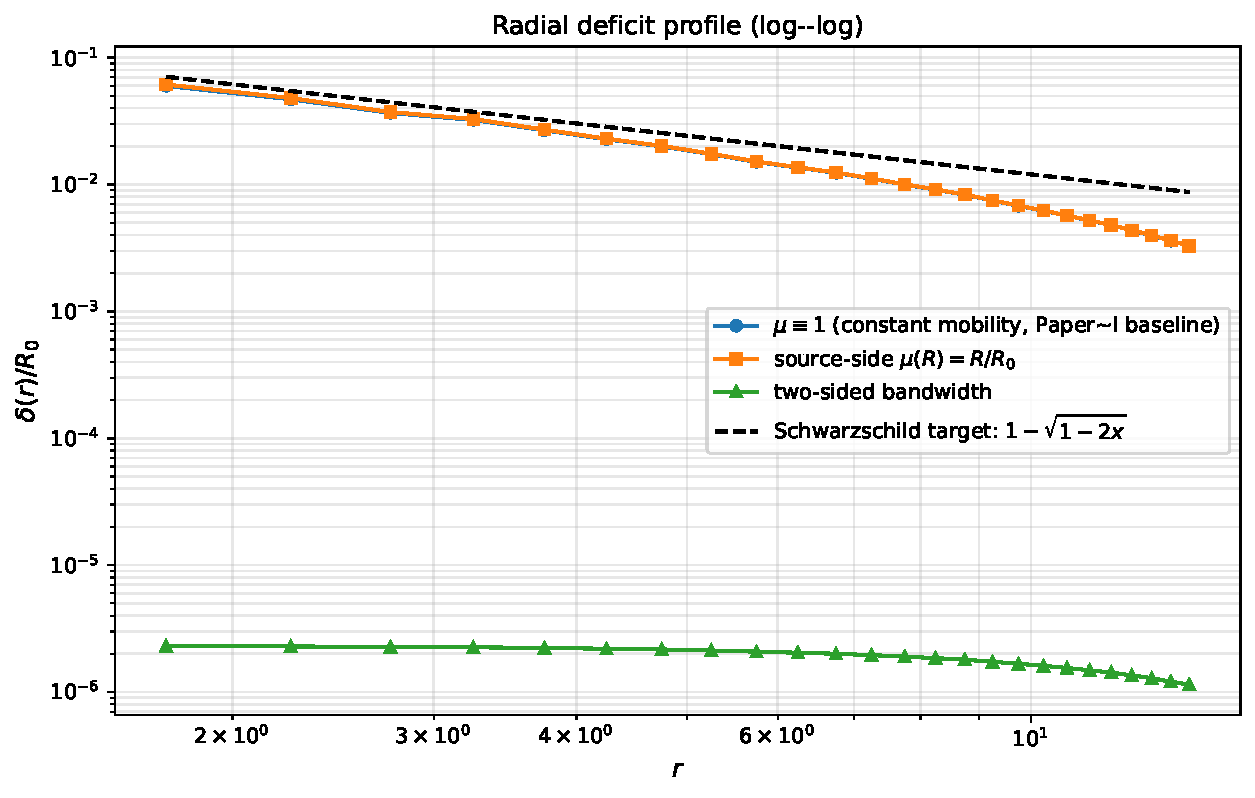
\includegraphics[width=0.92\textwidth]{figures/fig4a_cascade_profile.pdf}
\caption{Radial deficit profile $\delta(r)/R_0$ around a
single sink, on a cubic substrate of side $L = 32$ at sink
strength $E_0 = 1.5$,
time step $\tau = 0.05$, $n_{\text{ticks}} = 5000$, plotted log--log. Three mobility
choices are shown: constant mobility $\mu \equiv 1$ (the
baseline of Paper~I), the source-side bandwidth mobility
$\mu(R) = R/R_0$, and the two-sided bandwidth prescription.
The dashed black curve is the continuum Schwarzschild
clock-rate target $1 - \sqrt{1 - 2x}$ with
$x = M_{\rm eff}/(4\pi r R_0)$. The two-sided prescription
freezes near the sink, as discussed in
Sec.~\ref{sec:numerical}.}
\label{fig:cascade-profile}
\end{figure}

\begin{figure}[t]
\centering
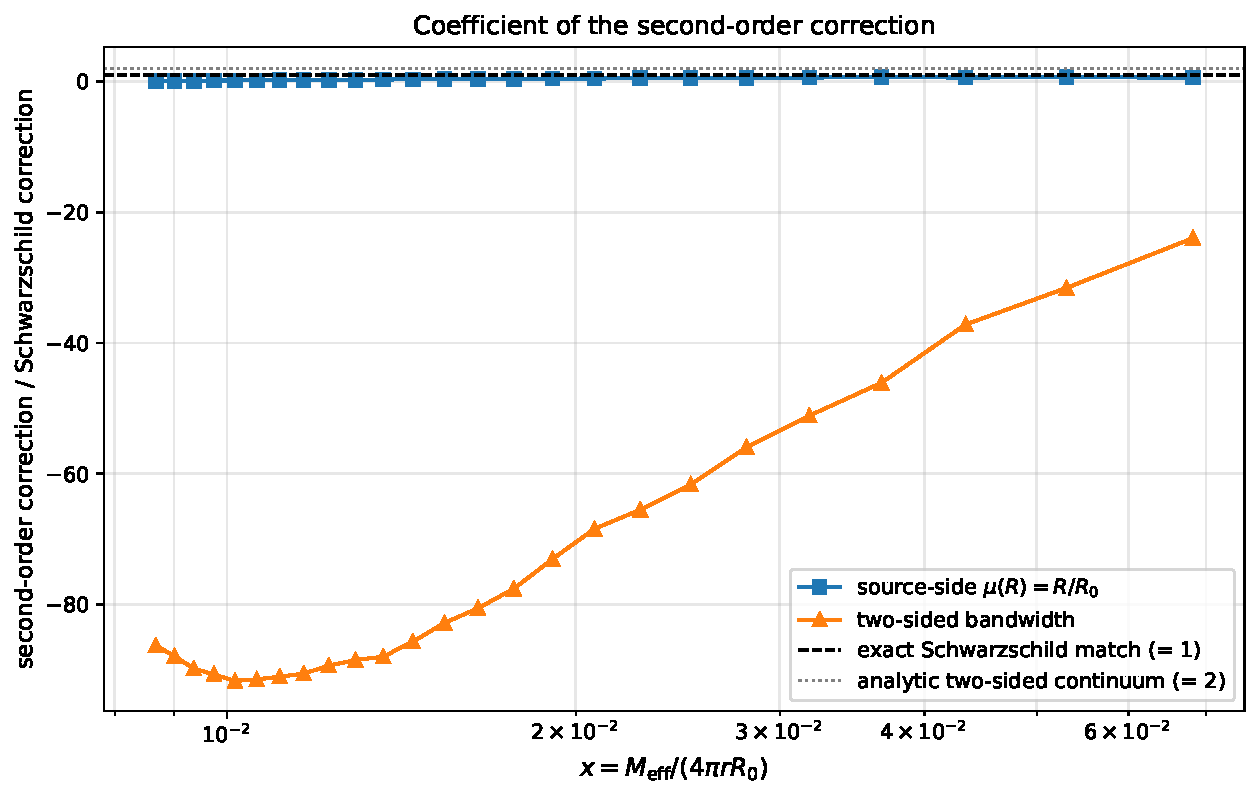
\includegraphics[width=0.92\textwidth]{figures/fig4b_cascade_correction.pdf}
\caption{Coefficient of the second-order correction added by
each mobility choice, normalised to the Schwarzschild
correction $\delta_{\rm Schw} - x$. The dashed line at $1$ is
the exact Schwarzschild match for the source-side prescription;
the dotted line at $2$ is the analytic continuum prediction for
the two-sided prescription (where $R/R_0 = (1-B/r)^{1/3}$
expands with prefactor $2$ at second order). \emph{The
source-side bandwidth mobility approaches $1$ at small $x$,
within lattice resolution and confirms the analytic match. The
two-sided curve is plotted on the same axis but is dominated by
the cascade-freezing pathology of Sec.~\ref{sec:numerical}: it
diverges from the continuum prediction far from the analytic
$+2$ value, which is the empirical signature that the two-sided
prescription leaves the small-displacement linear regime well
before the source-side prescription does.} The two-sided curve
should accordingly be read as a null-hypothesis comparator
illustrating the cascade-collapse pathology, not as a
verification of the continuum $+2$ coefficient.}
\label{fig:cascade-correction}
\end{figure}

\section{Calibration vs.\ prediction}
\label{sec:cal-vs-pred}

We separate clearly:

\textbf{Inputs (assumed, not derived).}
\begin{itemize}
\item Bandwidth identification \eqref{eq:tau_def}: an
operational hypothesis. It states that the local rate of
effective proper time at a node is its available reserve,
normalised to $R_0$.
\item Source-side bandwidth mobility $\mu(R) = R/R_0$,
Eq.~\eqref{eq:throttle}: derived in Sec.~\ref{sec:axiomatic-derivation}
within the additive local-capacity framework. The remaining
physical assumption is the additivity axiom (L4); alternative
non-additive capacity laws define different theories and
generally yield different radial profiles.
\item $M_{\rm eff} / R_0 \leftrightarrow 2 G M_{\rm phys} / c^2$:
fixes one combination of lattice unit and rest level by
demanding the leading-order deficit match the Newtonian
potential. Inherited from Paper~I.
\end{itemize}

\textbf{Derived from these inputs.}
\begin{itemize}
\item The functional form $R/R_0 = \sqrt{1 - 2GM/c^2 r}$ as
the unique spherically symmetric, steady-state solution of the
continuum equation $\nabla^2(R^2) = 0$ with $R \to R_0$ at
infinity, given the source strength.
\item The location of the bandwidth horizon, $r = 2GM/c^2$,
as the locus where $R = 0$ in this solution.
\item The flux conservation law $\kappa E_0 = 2 \pi \alpha
R_0 \beta$ relating source strength to the integrated flux
across any sphere outside the sink.
\item The structural form of Newton's gravitational constant
$G$ as a function of $(\kappa, \alpha, R_0, d_{\min},
\varepsilon_{\rm latt})$, together with a single Planck-scale
dimensionless constraint, $\kappa/(\alpha R_0) = 4\pi$
(Sec.~\ref{sec:newton-G}). The numerical value of $G$ is not
predicted; the structural form is.
\end{itemize}

\section{Structural form of Newton's constant}
\label{sec:newton-G}

The mobility framework gives more than the Schwarzschild form:
it fixes the dependence of Newton's gravitational constant $G$
on the local-rule parameters. We do not predict the SI value of
$G$ (that requires an external anchoring of the lattice scale),
but we derive its functional form, verify the predicted scaling
numerically, and show that under Planck-scale anchoring the
local rule must satisfy a single dimensionless relation.

\subsection{Mass--energy mapping and the form of $G$}

Convert the lattice source intensity $E_0$ to a physical energy
through the lattice-to-physical unit $\varepsilon_{\rm latt}$,
\begin{equation}
M \;=\; \frac{\mathcal{E}_{\rm src}}{c^2}
   \;=\; \frac{E_0\,\varepsilon_{\rm latt}}{c^2},
\label{eq:mass_def}
\end{equation}
and the lattice $\beta$ to a physical length through the
lattice spacing $d_{\min}$, $\beta_{\rm phys} = \beta\,
d_{\min}$. Substituting Eq.~\eqref{eq:beta_def} into the
calibration $\beta_{\rm phys} = 2GM/c^2$ gives
\begin{equation}
\frac{2GM}{c^2}
\;=\; \frac{\kappa\, E_0\, d_{\min}}{2\pi\, \alpha\, R_0},
\end{equation}
which combined with Eq.~\eqref{eq:mass_def} yields
\begin{equation}
\boxed{\;
G \;=\; \frac{\kappa\, c^4\, d_{\min}}
              {4\pi\, \alpha\, R_0\, \varepsilon_{\rm latt}}.
\;}
\label{eq:G_form}
\end{equation}
Three remarks. (i)~The combination of $(\kappa, \alpha, R_0)$
that enters $G$ is the dimensionless ratio $\kappa/(\alpha
R_0)$ alone --- the rule has only one structural degree of
freedom relevant to $G$. (ii)~The lattice scale
$d_{\min}/\varepsilon_{\rm latt}$ enters as an overall
multiplicative factor not determined by the local rule.
(iii)~The dimensional structure $[G] = L\,c^4/E$ is reproduced
without additional postulates.

\subsection{Numerical verification of the scaling}

We test the prediction Eq.~\eqref{eq:beta_def} by varying each
parameter $(\kappa, \alpha, R_0, E_0)$ independently and
extracting $\beta$ from the inner-shell measurement
$\beta = 2 r [1 - (R(r)/R_0)^2]$ at $r = 3$ along a principal
axis, on $L = 24$ with $\tau = 0.05$ and $4000$ ticks
(\texttt{code/G\_parameter\_scan.py}).

\begin{table}[h]
\centering
\begin{tabular}{cccc}
\toprule
Parameter & Range & Predicted exponent & Measured exponent\\
\midrule
$\kappa$  & $0.5 \to 2.0$  & $+1$ & $+0.9999$\\
$\alpha$  & $0.5 \to 2.0$  & $-1$ & $-0.9988$\\
$R_0$     & $0.7 \to 1.3$  & $-1$ & $-0.9999$\\
$E_0$     & $0.1 \to 0.5$  & $+1$ & $+0.9999$\\
\bottomrule
\end{tabular}
\caption{Scaling of $\beta$ under independent variation of
each parameter, on $L = 24$. All four predicted exponents are
recovered to better than $0.2\%$. The constant ratio
$\beta_{\rm meas}/\beta_{\rm pred} \approx 0.807$ across all
scans is the finite-volume Madelung correction at this lattice
size; it is the same multiplicative factor in every scan and
does not affect the scaling. Data: \texttt{data/G\_parameter
\_scan.json}.}
\label{tab:G_scaling}
\end{table}

The $\alpha$ exponent is recovered cleanly across the full
range. In a pre-mobility convention with a hard flux cap, this
scan was broken at large $\alpha$ because the cap clipped the
flux before the cascade reached steady state; under the
mobility framework the flux bound follows automatically from
$R \ge 0$ and the rate-limiter $\beta_i$, and the scan is
clean.

\subsection{Planck-scale anchoring}

Identifying the lattice scale with the Planck scale,
\[
d_{\min} \equiv \ell_P = \sqrt{\hbar G / c^3},
\qquad
\varepsilon_{\rm latt} \equiv E_P = \sqrt{\hbar c^5 / G},
\]
and substituting in Eq.~\eqref{eq:G_form}, with $\hbar = c = 1$
in Planck units, one obtains
\begin{equation}
\boxed{\;
\frac{\kappa}{\alpha\, R_0} \;=\; 4\pi
\quad
\text{(in Planck units, $\hbar = c = 1$).}
\;}
\label{eq:Planck_constraint}
\end{equation}
Under the identification of the lattice scale with the Planck
scale, the local-rule parameters must satisfy this single
dimensionless relation in order to recover the experimentally
measured value of $G$. This is a \emph{consistency check},
not a first-principles prediction: the numerical value of $G$
requires external Planck-scale anchoring as discussed in
Sec.~\ref{sec:cal-vs-pred}. The
simulation parameters $\kappa = \alpha = R_0 = 1$ used
throughout this paper are scaled for numerical convenience and
do not satisfy Eq.~\eqref{eq:Planck_constraint} numerically;
the physical lattice anchored at the Planck scale would.

\subsection{Honest accounting and the parameter count}

Equation~\eqref{eq:Planck_constraint} is a calibration
condition --- it matches the CODATA value of $G$ given the
Planck-scale identification of $d_{\min}$ and
$\varepsilon_{\rm latt}$ --- not a first-principles
prediction. The structural form Eq.~\eqref{eq:G_form} is
derived from the rule; the numerical value of $G$ requires the
external Planck-scale identification.

The parameter count of the rule decreases under the mobility
framework. An earlier formulation (now archived; see
Sec.~\ref{sec:code}) carried a separate capacity field $\chi$
in addition to the reserve $R$, and three parameters
$(\kappa, \alpha, \chi_0)$ entered $G$ through the combination
$\kappa\, \chi_0^2 / \alpha$. The mobility framework
eliminates $\chi$ as a structural variable, and only $\kappa /
(\alpha R_0)$ enters $G$. At fixed normalisation $R_0$ this is
one effective parameter. One residual freedom remains, which
we expect to be fixed by an analogous calibration in the
oriented-flux (electromagnetic) sector deferred to a later
paper.

\paragraph{Calibration ledger (per SERIES\_FEEDBACK §0.ter).}
Each quantity in this paper falls into one of three statuses
per §0.ter: \emph{derived} from substrate principles +
hypotheses, \emph{hypothesised} as a labelled structural choice,
or \emph{calibrated} against an empirical reference (SM/GR
result or CODATA constant). The status of each new quantity
introduced in this paper is summarised below.
The present paper extends Paper~I. The following table lists
the new quantities and their status:

\begin{center}
\begin{tabular}{p{3.4cm}p{3.0cm}p{6.6cm}}
\toprule
Quantity & Status & Calibration source / future resolution \\
\midrule
$\mu(R) = R/R_0$ & hypothesis (closed under axioms (L1)--(L4)) & sub-hypothesis of (H-mobility); origin open \\
(L4) additive capacity (H1) & axiom + open problem (O1) & not derived; future microscopic argument \\
$d\tau/dt = R/R_0$ (H2) & hypothesis (open problem (O2)) & operational identification; future derivation \\
$\beta = 2GM/c^2$ & calibrated & SM/GR Newtonian limit identification; future microscopic origin \\
Newton's $G$ (physical units) & calibrated & CODATA recommended value via Planck anchoring \\
$\kappa/(\alpha R_0) = 4\pi$ & consistency check & derived constraint among lattice parameters \\
$R/R_0 = \sqrt{1-\beta/r}$ & derived & from (L1)--(L4) + (H1) + (H2) in continuum limit \\
\bottomrule
\end{tabular}
\end{center}

\paragraph{Rule loci touched and no-epicycle statement (per SERIES\_FEEDBACK §0.quater).}
This paper extends Paper~I at the following loci, and at no
other:
\begin{itemize}
\item \emph{Update rule:} the constant-mobility baseline
$\mu \equiv 1$ of Paper~I is replaced by the source-side
bandwidth-throttled choice $\mu(R) = R/R_0$ (Sec.~\ref{sec:axiomatic-derivation}).
This is a labelled within-locus extension, not a new locus.
\item \emph{Configuration:} the point sink of Paper~I is
specialised to a static spherically-symmetric source.
\end{itemize}
Nodes, links, substrate topology and update structure are
otherwise inherited from Paper~I unchanged.

\noindent\emph{No-epicycle statement.} No new fields on nodes
or links, no new parameters beyond those listed in the
calibration ledger, and no relaxation of (L1)--(L6) of Paper~I
have been silently introduced. The Schwarzschild form
emerges from the labelled hypotheses (H1) and (H2) without
additional structural ingredients.

\section{Limitations and scope}
\label{sec:not}

We do not derive the Schwarzschild form for non-spherical or
non-static configurations. The derivation in
Sec.~\ref{sec:derivation} uses spherical symmetry and steady
state. Rotating, oscillating, or multi-source configurations
are not covered.

We do not derive the spatial part of the Schwarzschild metric.
The derivation gives the $g_{00}$ factor only. The radial
component, the angular components, the propagation of light
through the modified bandwidth field, and any other component
of the metric structure are not addressed.

We do not derive the Einstein field equations. The dynamical
content of GR --- the Bianchi identities, the matter coupling,
the propagation of gravitational waves --- is outside the
scope of this paper.

We do not derive the additivity axiom (L4) from deeper
substrate microphysics. What
Sec.~\ref{sec:axiomatic-derivation} establishes is narrower:
within the class of regular local emission-capacity rules
satisfying locality, internal conservation, empty-reserve
extinction, rest-state normalisation, and additive composition
of independent reserve packets, the source-side mobility is
uniquely selected as $\mu(R) = R/R_0$. Thus the remaining open
assumption is not the mobility function itself, but the
microscopic origin of additive emission capacity.

We do not address kinematic time dilation. The motion of a
localised configuration across the substrate, and any
relationship to the special-relativistic Lorentz factor, is
the subject of Paper~III.

We do not predict the SI value of Newton's $G$. The structural
form of $G$ in terms of the local-rule parameters is derived
in Sec.~\ref{sec:newton-G}, but the absolute lattice scale must
be anchored externally. The speed of light $c$ enters as a
calibration, exactly as in Paper~I.

\section{Relation to existing work}
\label{sec:related}

\textbf{Weak-field general relativity.} The match
\eqref{eq:dtau_schw} reproduces the static Schwarzschild
clock-rate factor as a formal function of $GM/c^2 r$. The
leading order is calibration-mediated and coincides with the
Newtonian limit; the higher-order terms follow from the
bandwidth-throttled cascade. Within this model, we identify a
$g_{00}$-like quantity only; we do not derive the spatial part
of the Schwarzschild metric, the Einstein field equations, or
weak-field GR more generally.

\textbf{Emergent gravity programmes}
\cite{verlinde2011,padmanabhan2010,jacobson1995}. These
derive gravitational behaviour from thermodynamic or
information-theoretic arguments on horizons. The present
paper operates at a different level: an explicit local rule
with an explicit throttle prescription, rather than a
coarse-grained thermodynamic identity. The two are not in
competition; they target different levels of description.

\textbf{Lattice and discrete models of gravity}
\cite{benzi1992,wolfram2002,thooft2016,regge1961,ambjorn2012cdt}. Lattice fluid models
recover continuum hydrodynamic equations through similar
steady-state and conservation arguments. The present paper
differs in two respects: the bandwidth identification
\eqref{eq:tau_def} maps the substrate's flux activity onto
local proper time, which is, to our knowledge, not adopted in
the same form within the local-rule programme; and the
source-side bandwidth mobility is the specific structural
ingredient that produces $\nabla^2(R^2) = 0$ rather than
$\nabla^2 R = 0$, upgrading the constant-mobility $1/r$ profile
of Paper~I to the Schwarzschild static clock-rate factor in the
spherical sector.

\section{Code and data availability}
\label{sec:code}

The Python script \texttt{code/iterative\_cascade\_test.py}
implements the rule of Paper~I with three mobility choices
(constant, source-side $\mu = R/R_0$, two-sided
$\mu(R_i)\mu(R_j) = R_i R_j / R_0^2$) and produces the radial
profiles of Sec.~\ref{sec:numerical}. The script
\texttt{code/G\_parameter\_scan.py} performs the parameter
scan of Sec.~\ref{sec:newton-G}, varying $(\kappa, \alpha,
R_0, E_0)$ independently and verifying the predicted scaling
exponents. Both scripts are pure-numpy and depend on no
external simulation framework. The numerical data of
Tables~\ref{tab:cascade}, \ref{tab:schw_match}, and
\ref{tab:G_scaling} are stored in
\texttt{data/iterative\_cascade\_L40.json} and
\texttt{data/G\_parameter\_scan.json}. The repository is
available at
\url{https://github.com/stanislasdewavrin/DDD-Paper-2-Gravity}.

\paragraph{Archived material on the form of $G$.}
An earlier standalone draft used a separate capacity field
$\chi$ in addition to the reserve $R$. Its derivation has been
absorbed into Sec.~\ref{sec:newton-G} of the present paper
under the simpler mobility framework, and its remaining
content (extended discussion of the dimensionless constraint,
comparison with emergent-gravity programmes, draft material
for the constants-and-hierarchies paper) is archived under
\texttt{paperXV\_constants/draft\_material/}.

\section{Principal open problems}
\label{sec:open}

The following two gaps are of equal logical weight and control
distinct structural features of the construction: (O1)
constrains the mobility selection, while (O2) constrains the
proper-time identification. Both are co-equal principal open
problems; neither is reducible to the other.

\paragraph{(O1) Origin of the additivity axiom (L4).}
Sec.~\ref{sec:axiomatic-derivation} derives $\mu(R) = R/R_0$
from the additive-capacity axiom (L4), but does not derive (L4)
itself from deeper substrate microphysics. (L4) encodes the
physical content that the substrate has no hidden saturation
between independent reserve packets at sub-rest scales; a
microscopic explanation of why independent reserve packets
compose additively in the local emission-capacity envelope
would close the remaining gap. We state this as the principal
open problem of the present construction rather than as a
defended position; alternative non-additive capacity laws
define different theories whose own falsifiable predictions
could in turn be tested against data.

\paragraph{(O2) Origin of the bandwidth identification (H2).}
The identification of effective proper time with the
reserve-normalised bandwidth (Eq.~\eqref{eq:tau_def}) is
operational and labelled (H2). It is the second substantive
hypothesis of the construction, on the same logical footing as
the additivity axiom (L4): both are not derived from substrate
microphysics, both control structurally distinct features of
the result (mobility selection vs. proper-time identification),
and a uniqueness/microscopic argument for either would
strengthen the construction by an independent route.

A microscopic argument that selects the linear dependence
\eqref{eq:tau_def} from the rule, or that establishes proper
time as a derived rather than adopted quantity, would close
this gap. Candidate routes include: (i) a uniqueness theorem
on the form of the local rate-of-events functional under
locality, conservation and isotropy; (ii) a renormalisation-group
argument selecting a power-law fixed point at exponent 1; or
(iii) a direct derivation from a discrete-time observer
clock construction. We state (H2) as a principal open problem
on equal footing with (L4); alternative identifications
$d\tau/dt = (R/R_0)^p$ with $p \ne 1$ define different theories
whose predictions diverge from Schwarzschild and could be
falsified by precision tests.

\paragraph{Beyond the linear regime: rate-limiter and
bandwidth horizon.} When a node's reserve approaches zero (near
the bandwidth horizon $r = \beta$, where $R \to 0$), the
discrete rate-limiter $\beta_i \in [0,1]$ of Paper~I --- which
caps outflows to enforce $R_i \ge 0$ --- becomes active and
the rule departs from the linearised regime. This discrete
saturation enforcement is not derivable from the continuum
equation alone: it is a lattice-scale feature that stabilises
the solution on finite lattices (analogous to a UV regulator)
and protects against spurious singularities of the continuum
square-root form. The interplay between
the continuum square-root singularity $R \propto \sqrt{1 -
\beta/r}$ and the discrete saturation enforcement is not
addressed in the present paper: a numerical study of
convergence as $L \to \infty$ approaching the horizon, and a
physical interpretation of the rate-limiter as a
substrate-scale regulator (analogous to a UV cutoff), would
clarify the model's structure near $r = 2GM/c^2$. We expect
the rate-limiter to render the rule well-defined for all
$r > 0$ on a finite lattice; the continuum behaviour at and
inside the horizon is not derived here. Note also a notation
overlap: the symbol $\beta$ is used both for the deficit
parameter (Eq.~\eqref{eq:profile}, here a length scale) and,
in Paper~I, for the discrete rate-limiter $\beta_i$ (a
dimensionless cap); these are distinct objects.

\paragraph{Spatial part of the metric.}
The bandwidth identification gives $g_{00}$. Whether the
substrate also produces a consistent spatial metric, and
whether photon trajectories computed from the bandwidth field
reproduce the deflection angle $4GM/c^2 b$ of weak-field GR,
is the subject of Paper~IV.

\paragraph{Back-reaction.} The probe approximation ignores
the test configuration's contribution to the deficit field.
The full self-consistent treatment is also left to Paper~IV.

\section{Outlook}
\label{sec:outlook}

The companion papers extend the substrate of Paper~I along several
axes; this paper covers the static spherical gravitational sector
only. The structure of the rest of the series is:

\begin{enumerate}
\item \textbf{Paper~III} --- a Floquet two-step spinor sector on the
same substrate supports propagating localised excitations and an
operational, kinematic Lorentz-like clock-rate. Provides the
relativistic kinematics that complement this paper's
gravitational sector.
\item \textbf{Paper~IV} --- calibrates the photon-substrate coupling
against the static spherical regime developed here, and reproduces
light deflection and Shapiro delay at the percent level. Closes
the canonical solar-system tests of GR.
\item \textbf{Paper~V} --- collects falsification windows of the
gravitational sector: short-range Yukawa screening (E\"ot--Wash),
post-Newtonian deviations from $C_{\rm PPN}$, ultra-relativistic
Lorentz windows, compact-object near-horizon phenomenology.
\item \textbf{Paper~VI} --- extends the substrate with a compact U(1)
oriented sector; derives Maxwell-like dynamics in the weak-field
limit and proposes a candidate fixed-point formula for
$\alpha_{\rm EM} \simeq 1/137$.
\item \textbf{Paper~VII} --- studies the joint Wilson-loop
back-reaction of gravity and electromagnetism at the substrate
scale, predicting $\alpha_G/\alpha_{\rm EM} = 1/\sqrt{2}$,
$m_{\rm lat} \approx 0.072\,M_P$, and cross-coupling consequences
observable in atomic clocks and cosmological $\dot\alpha/\alpha$.
\item \textbf{Paper~VIII} --- the cosmogenetic regime
($R_i \to 0$ initial state with a single founding impulse)
reproduces the DESI DR2 evolving dark-energy signal.
\end{enumerate}

The principal open task of the present paper is to derive the
additivity axiom (L4) from deeper substrate microphysics, rather
than adopting it as the substantive postulate that closes the
emission-capacity class. Until that is done, the
Schwarzschild-like clock-rate factor of
Eq.~\eqref{eq:dtau_schw} should be read as a consequence of the
additive local-capacity framework
(Sec.~\ref{sec:axiomatic-derivation}) and the
bandwidth-identification hypothesis
(Sec.~\ref{sec:claims}, Claim~1).

\bibliographystyle{unsrt}
\bibliography{references}


\paragraph{Closing reaffirmation (analogue framing).}
To reiterate: this paper recovers the \emph{form} of the
Schwarzschild static clock-rate factor inside an analogue
substrate, not a derivation of General Relativity itself. The
result is internal to the analogue and conditional on
hypotheses (H1) additivity and (H2) bandwidth identification.
GR remains the empirical anchor; any deviation between the
analogue and measured tests of GR falsifies the analogue, not
GR.

\end{document}
